\section{From Classical Prediction to Representation Learning}

The previous sections developed a general mathematical view of learning: data define a task, losses define performance, model classes encode inductive bias, and optimization turns an objective into a learned predictor. We now arrive at a transition that is historically and conceptually decisive.

For a long time, much of machine learning was organized around the following pattern: first design features by hand, then learn a predictor on top of those features. Modern deep learning changed this pattern by making the features themselves learnable.

This shift from \emph{fixed representations} to \emph{learned representations} is one of the central ideas of the book.

\subsection*{Representations as internal coordinate systems}

A predictor need not act directly on raw inputs. Often, the input is first transformed into a new space in which the relevant structure is easier to express.

\begin{definition}[Representation map]
A \emph{representation map} is a function
\[
\phi:\mathcal X\to\mathcal Z
\]
from the input space $\mathcal X$ to a feature or representation space $\mathcal Z$. The image $\phi(x)$ is called a \emph{representation} or \emph{feature vector} of the input $x$.
\end{definition}

The point of a representation is not merely to re-encode the data, but to place them in coordinates that make the downstream task simpler. A good representation can separate classes, reveal latent structure, or compress information while retaining what matters for prediction.

\subsection*{Classical learning as prediction on fixed features}

Many classical learning pipelines can be written in the compositional form
\[
f = g\circ \phi,
\]
where $\phi$ is a feature map and $g$ is a predictor acting on the feature space.

\begin{proposition}[Classical learning often uses a fixed representation]
In many classical learning methods, prediction takes the form
\[
f(x)=g(\phi(x)),
\]
where the representation map $\phi:\mathcal X\to\mathcal Z$ is fixed before learning, and only the predictor $g:\mathcal Z\to\mathcal Y$ is learned from data.
\end{proposition}

\begin{proof}
The statement is structural rather than tied to one algorithm. In a classical pipeline, one first defines features
\[
z=\phi(x),
\]
for example edge counts, frequency statistics, polynomial expansions, or kernel-induced coordinates. One then applies a learned predictor $g$ to those features:
\[
\hat y = g(z)=g(\phi(x)).
\]
Because the feature map is specified in advance and not adapted through training, the learned part of the system is $g$, not $\phi$.
\end{proof}

Examples include:

\begin{itemize}
    \item linear regression on manually engineered input features,
    \item support vector machines on hand-crafted descriptors,
    \item classifiers built on signal-processing features such as MFCCs in speech or SIFT-like descriptors in vision,
    \item kernel methods in which the representation is determined implicitly by the choice of kernel.
\end{itemize}

The important point is not that these methods are weak; many are extremely powerful. The point is that the representational stage is largely external to the learning process.

\begin{figure}[tbp]
\centering
\begin{tikzpicture}[
    box/.style={draw, rounded corners, fill=gray!10, inner sep=6pt, minimum width=3cm, minimum height=1cm},
    arrow/.style={-{Latex[length=2.2mm]}, thick},
    every node/.style={align=center}
]
\node[box] (raw) at (0,0) {raw input\\$x\in\mathcal X$};
\node[box] (feat) at (4.2,0) {hand-crafted features\\$\phi(x)\in\mathcal Z$};
\node[box] (pred) at (8.4,0) {learned predictor\\$g:\mathcal Z\to\mathcal Y$};
\node[box] (out) at (12.6,0) {prediction\\$\hat y=g(\phi(x))$};

\draw[arrow] (1.55,0) -- (2.65,0);
\draw[arrow] (5.75,0) -- (6.85,0);
\draw[arrow] (9.95,0) -- (11.05,0);

\node at (4.2,-1.05) {\small chosen by the designer};
\node at (8.4,-1.05) {\small fit from data};
\end{tikzpicture}
\caption{A classical pipeline: raw inputs are first converted into hand-crafted features, and a learned predictor is trained on top of those fixed features.}
\end{figure}

\subsection*{Why representations matter}

The same predictor class can behave very differently depending on the representation. A linear classifier may fail completely in raw coordinates and succeed immediately in a more suitable feature space.

This is one reason feature design mattered so much in classical machine learning: the choice of representation often determined whether the learning problem became simple or difficult.

At a conceptual level, the representation map $\phi$ acts as an \emph{internal coordinate system}. It changes the geometry of the problem. Distances, linear separability, smoothness, and cluster structure may look very different in $\mathcal Z$ than in $\mathcal X$.

\subsection*{Deep learning as representation learning}

Modern deep learning changed the balance of the pipeline by making the representation itself adaptive.

\begin{proposition}[Deep learning makes the representation learnable]
A deep learning model typically has the compositional form
\[
f_\theta = g_{\theta_2}\circ \phi_{\theta_1},
\]
or more generally
\[
f_\theta = h_L\circ h_{L-1}\circ \cdots \circ h_1,
\]
where the representation map is parameterized and learned from data together with the final predictor.
\end{proposition}

\begin{proof}
In a multilayer model, each intermediate map transforms its input into a new representation:
\[
z_1=h_1(x),\qquad z_2=h_2(z_1),\qquad \dots,\qquad z_L=h_L(z_{L-1}).
\]
The final prediction is obtained by composition. Because the parameters of these layers are updated during training, the intermediate representations are not fixed in advance. They are learned jointly with the output map in order to reduce the training objective.
\end{proof}

This is the decisive conceptual shift. Instead of asking only, ``Which predictor should be fit on top of a feature space?'', deep learning asks, ``Which feature space should itself be learned so that prediction becomes easier?''

\begin{figure}[tbp]
\centering
\begin{tikzpicture}[
    box/.style={draw, rounded corners, fill=gray!10, inner sep=6pt, minimum width=2.55cm, minimum height=1cm},
    arrow/.style={-{Latex[length=2.2mm]}, thick},
    every node/.style={align=center}
]
\node[box] (raw) at (0,0) {raw input\\$x$};
\node[box] (h1) at (3.2,0) {layer 1\\$z_1=h_1(x)$};
\node[box] (h2) at (6.4,0) {layer 2\\$z_2=h_2(z_1)$};
\node[box] (h3) at (9.6,0) {layer 3\\$z_3=h_3(z_2)$};
\node[box] (out) at (12.8,0) {predictor\\$\hat y=h_4(z_3)$};

\draw[arrow] (1.25,0) -- (1.95,0);
\draw[arrow] (4.45,0) -- (5.15,0);
\draw[arrow] (7.65,0) -- (8.35,0);
\draw[arrow] (10.85,0) -- (11.55,0);

\node at (6.4,-1.05) {\small representations are learned jointly across layers};
\end{tikzpicture}
\caption{A deep learning pipeline: the representation is not fixed in advance but built through multiple learned transformations.}
\end{figure}

\subsection*{A worked example: raw inputs, hand-crafted features, and learned hidden representations}

Consider a binary classification problem in $\mathbb R^2$ where the positive class lies near a ring around the origin and the negative class lies near the center. In raw coordinates, these classes are not linearly separable.

\paragraph{Raw-input linear classifier.}
A linear classifier has the form
\[
f(x)=\operatorname{sign}(w^\top x+b).
\]
Because its decision boundary is a line, it cannot separate a central cluster from a surrounding ring.

\paragraph{Hand-crafted feature representation.}
Now define a feature map
\[
\phi(x)=\|x\|^2=x_1^2+x_2^2.
\]
A linear rule in feature space becomes
\[
g(\phi(x))=\operatorname{sign}(a\,\phi(x)+c),
\]
which is equivalent to thresholding the squared radius. This can separate the inner cluster from the outer ring.

\paragraph{Learned hidden representation.}
A multilayer neural network may instead learn an internal map
\[
\phi_\theta:\mathbb R^2\to\mathbb R^m
\]
such that the transformed points become approximately linearly separable in representation space. The final layer may still be linear,
\[
\hat y = \operatorname{sign}(w^\top \phi_\theta(x)+b),
\]
but now the coordinates have been learned rather than manually designed.

The lesson is not merely that neural networks are more flexible. It is that deep learning moves feature construction inside the learning process.

\begin{figure}[tbp]
\centering
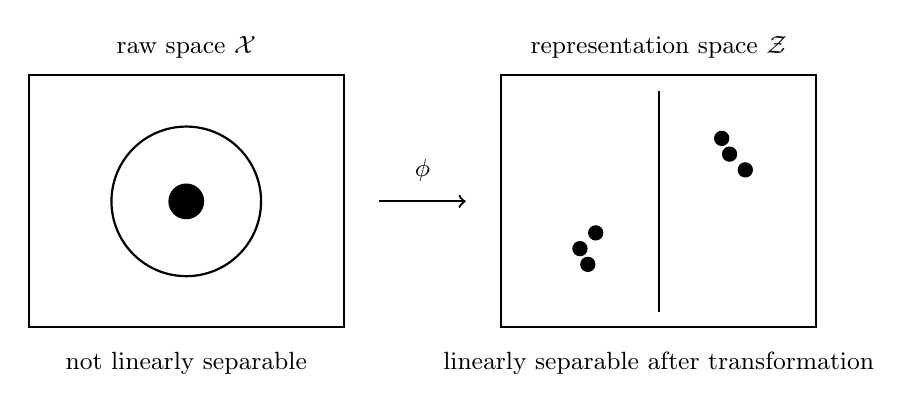
\begin{tikzpicture}[scale=1, every node/.style={align=center}]
    % left plot
    \draw[thick] (0,0) rectangle (4,3.2);
    \node at (2,3.55) {\small raw space $\mathcal X$};
    \draw[thick] (2,1.6) circle (0.95);
    \filldraw (2,1.6) circle (0.22);
    \node at (2,-0.45) {\small not linearly separable};

    % right plot
    \draw[thick] (6,0) rectangle (10,3.2);
    \node at (8,3.55) {\small representation space $\mathcal Z$};
    \filldraw (7.0,1.0) circle (0.09);
    \filldraw (7.2,1.2) circle (0.09);
    \filldraw (7.1,0.8) circle (0.09);
    \filldraw (8.9,2.2) circle (0.09);
    \filldraw (9.1,2.0) circle (0.09);
    \filldraw (8.8,2.4) circle (0.09);
    \draw[thick] (8,0.2) -- (8,3.0);
    \node at (8,-0.45) {\small linearly separable after transformation};

    \draw[->, thick] (4.45,1.6) -- (5.55,1.6);
    \node at (5,2.0) {\small $\phi$};
\end{tikzpicture}
\caption{A schematic feature-space view. In raw coordinates, the relevant classes may be entangled, while an appropriate representation can transform them into a space where a simple decision rule becomes effective.}
\end{figure}

\subsection*{Representation learning as the deep-learning successor to feature engineering}

This perspective helps connect classical and modern machine learning.

In classical methods, the designer often supplied the structure:
\[
x \longmapsto \phi(x) \longmapsto g(\phi(x)).
\]
In deep learning, the model seeks that structure from data:
\[
x \longmapsto \phi_{\theta_1}(x) \longmapsto g_{\theta_2}(\phi_{\theta_1}(x)).
\]

Thus architecture takes over part of the role once played by manual feature engineering. Convolutions encode locality and translation structure. Sequence models encode temporal dependence. Attention mechanisms encode content-based interaction. The model class does not only specify how to predict; it also specifies how useful representations may be constructed.

\commonconfusion{Representation learning does not mean that raw inputs become irrelevant or that hand-crafted structure disappears entirely. Deep models still rely on inductive bias: architecture, normalization, optimization, and data design all matter. The difference is that many useful intermediate features are now learned jointly with the task, rather than fixed completely in advance.}

\whattoremember{A representation map $\phi:\mathcal X\to\mathcal Z$ transforms raw inputs into coordinates better suited to a task. Classical learning often has the form $f=g\circ\phi$ with a fixed feature map $\phi$ and a learned predictor $g$. Deep learning changes this by making $\phi$ itself parameterized and learnable, often through many layers of composition. This shift from fixed features to learned representations is one of the defining ideas of modern machine learning.}

\subsection*{Exercises}

\begin{exercise}
Give an example of a learning problem in which a simple predictor becomes much more effective after a suitable feature transformation. Describe both the raw input space and the transformed feature space.
\end{exercise}

\begin{exercise}
Consider the feature map
\[
\phi(x_1,x_2)=(x_1,x_2,x_1^2+x_2^2).
\]
Explain why a linear classifier in the feature space can represent decision boundaries that are not linear in the original input space.
\end{exercise}

\begin{exercise}
In your own words, explain the difference between
\[
f(x)=g(\phi(x))
\]
with fixed $\phi$ and
\[
f_\theta(x)=g_{\theta_2}(\phi_{\theta_1}(x))
\]
with learned $\phi_{\theta_1}$.
\end{exercise}

\begin{exercise}
Why is it reasonable to say that representation learning changes the geometry of the problem? Give one example of a property that may become simpler in representation space than in raw space.
\end{exercise}

\begin{exercise}
A neural network ends with a linear output layer. Why is it still not ``just a linear model'' in general?
\end{exercise}

\subsection*{Notes and references}

This section marks the conceptual transition from classical prediction to deep learning. The central idea is that many learning systems can be written compositionally, but classical pipelines usually fix the representation map in advance, whereas deep learning makes that representation itself learnable. This is why the rise of neural networks was not only a change of model family but also a change in where feature construction occurs: it moved from external design into the learned system. The next chapter begins from exactly this question: if learning the representation is the key idea, what mathematical object is a neural network?